%% This is a lucky chapter (hence 13!) - being the first chapter that I will complete.
%% It combines the two previous chapters on Persistence (chpter5) and Stationarity (chpter4b)

See TODO list from chapter 5 (original persistence chapter).
%TODO: move the discussion/lit review on stability to somewhere useful
%
%TODO: These results also have trophic links between bottom and top levels. Need to re-run these simulations?
%TODO: Come back to this chapter having done work on stability... e.g. Are the presistent communtities stationary?
%TODO: Look at Thilo's reference on constructing stable GLM topologies (distinct pairs approach..)
%
%TODO: Are the 'good net' persistent net works here stationary??
%TODO: Find smaller stationary networks (4-10 species, and fit GLV!!) [w or w/o immigration]
%TODO: Finish All chapters on the IBM!!

% TODO: change path to figures in stationarity section?

\section{Temporary:context}

How does this chapter fit in with what has gone before and what follows:
\begin{itemize}
	\item Mention of `rescue effect' in previous chapter
	\item Desire to study changes in immigration rate (discussion of previous chapter)
	\item A good and convincing justification of the `default parameter set', and why we have used it up until now (and continue to use most of these values). 
	\item `community collapse' - define here or previously?
	
	\item The first figure (fractional persistence) is taken from chapter on varying immigration - check no duplication, and refer to it from there.
	
	\item Important: to state clearly that from now on we focus only on contiguous habitat loss (justify by realism, and time saving/focus)

	\item At some point we discover and remove vegetarian predators! (Which are allowed by the niche model) - probably when we also introduce the re-wiring algorithm.
	
	\item Make sure `functional groups have been introduced' - these are used here without explanation.
	
	\item Introduce the simulation ensembles HI, LI and NM1 (niche model) early on as they are used throughout the chapter. (Remove some of this description form the determinsim section, and the stationarity results section). Plot of NM1?!
\end{itemize}

%We first attempt to improve the persistence of our simulated communites by varying certain model parameters. The parameter space of the model is large (see table \ref{whereis}), therefore we do not attempt to explore all of it. Previous work by Lurgi et al. \cite{lurgi2015effects} in developing the model has ensured the realism of the bio-energetic parameters (where possisble they are derived from literature - more on this). Therefore we restrict our exploration to the region of the default parameters. 


\section{Introduction}

In the previous chapter we analysed in detail how simulated communities responded to two habitat loss scenarios. These simulations used the \emph{default parameter values} for the IBM model, as published in \cite{lurgi2015effects}. An important feature of these simulations was that they exhibited almost no species extinctions, even up to $90\%$ habitat loss (HL). This was achieved by a high immigration rate (IR), and was desirable because it allowed us to study underlying structural changes that were not associated with the loss of species. However, in nature the destruction or degradation of habitat often leads to a loss of species \cite{newbold2015global, foley2005global}. Therefore we also intend to use the model to investigate the regime where habitat loss causes extinctions. The obvious way to do this is to reduce the IR. Because this represents a departure from the default parameters and the way in which the model has been used previously, it requires a careful and systematic approach. Therefore in this chapter we `stress test' the model to analyse how it copes with changing IR. This is in preparation for chapter \ref{chap:varying_immigration_rate} where we will use this analysis as a foundation to study, from a more ecological perspective, how changing IR affects the response of communities to HL. In the first part of this chapter we look at \emph{closed communities} - what happens when there is no immigration? In the second part we address an issue that we discover arises from reduced IR, namely increased variability. In particular we focus on the concern that simulations may become dominated by stochastic effects, leading to unreliable results and loss of ecological meaning.

\section{Persistence in closed communities}
\label{sec:closed_communities}

We define a \emph{closed-community} as one in which there is no inflow of individuals from an external source. In the model this is achieved by setting the immigration rate to zero (IR$=0$). Here we study such communities in a pristine landscape - that is without habitat loss (HL$=0$). The simulation procedure is the same as in the previous chapter\footnote{Check where simulation procedure is described in detail.Chptr2?}. All parameters, except the IR, take default values unless otherwise stated, and each simulation uses a distinct network topology generated using the method outlined in chapter \ref{chap:habitat_loss_modelling_approach}. A species is said to \emph{persist} if there is at least one individual belonging to that species present in the landscape on the final iteration of the simulation\footnote{This may be a poor definition of persistence for a couple of reasons and we should discuss this later, possibly adopt a new definition in the next chapter.}. Therefore \emph{fractional persistence} is defined as the fraction of the initial pool of species (or subset of that pool) that persist\footnote{Discuss somewhere that this assumes steady-state: no guarantee that more species won't go extinct, or indeed `come back to life'}. ALSO MENTION NUMBER OF PERSISTENT SPECIES - THIS IS USED IN THE ANALYSIS.

An initial set of simulations with zero IR shows that species persistence is low (Figure \ref{fig:mvp_hist_zeroIR}). We see that for an antagonistic community (MAI$=0$) all non-basal species go extinct, as do around $30\%$ of basal species\footnote{Apparent competition? Over-grazing, due to lack of predators?}. Introducing mutualism into the communities slightly improves persistence in the higher trophic levels - we see some persistence of non-basal species, but no more than $10\%$ of the initial pool on average. So it seems that there is some small benefit of mutualism to the community as whole. However it is also clear that, given the default parameters, immigration is a requirement for the maintenance of species richness. In what follows we attempt to improve persistence in closed-communities and quantify the impact of varying sensibly chosen model parameters\footnote{Justify somewhere why are we attempting to improve persistence? Why do we care about persistence in closed communities?}. (Be more specific which sensibly chosen parameters are we varying?)

\begin{figure}
	\centering
	\includegraphics[width=0.8\linewidth]{"figures/persistence/hist_species_per_tl_zeroIR"}
	\caption{\textbf{Fractional persistence} by trophic level for three different MAI ratios, with \textbf{zero immigration} (IR=0). All other parameters set to default values. Fractional persistence is measured by the fraction of speices intially belonging to a trophic level which have not gone extinct by the end of a simulation (5000 iterations). The solid bars give the mean value, taken  from 22 repeat simulations. Error bars show $\pm$ one standard deviation.}
	\label{fig:mvp_hist_zeroIR}
\end{figure}

%\begin{figure}[h!]
%	\centering
%	\includegraphics[width=0.5\linewidth]{"figures/persistence/mvp1_22reps"}
%	\caption{Species persistence is plotted for 22 repeat simulations at each MAI ratio. Persistence is measured as the fraction of the initial 60 species that have not gone extinct by the end of a simulation (5000 iterations). Each blue dot gives the number of persistent species for a single simulation. The red line shows a linear regression fit with slope and p-value given in the inset.}
%	\label{fig:mai_vs_persistence}
%\end{figure}


\subsection{Mutualistic to antagonistic interaction (MAI) ratio}
\label{sec:mvp}

Mutualistic interactions are so named because they confer some benefit to both parties. One novel aspect of our modelling approach is the inclusion of mutualistic interactions into a spatial simulation of trophic dynamics, in a way that avoids Robert May's `orgy of mutual benefaction' \cite{may1981patterns} (see chapter \ref{chap:modelling_habitat_loss}). In \cite{lurgi2015effect} it was shown that increasing the levels of mutualism (MAI ratio) in the community can have a stabilising effect. However in the previous chapter we saw that this stability did not translate into a greater robustness of mutualistic communities to habitat loss. From figure \ref{fig:mvp_hist_zeroIR} we see that mutualism has a positive effect on persistence at zero IR. Therefore we explore this effect here.

An interesting feature of figure \ref{fig:mvp_hist_zeroIR} is that the benefit due to mutualism 

%A key theme throughout this thesis, and one of the main novel aspects of this research, is the inclusion of mutualistic interactions into simulated of trophic dynamics. In some cases we have seen that these mutualistic interactions play a stabilising role in the community (in contrast to May's classic `orgy of mutual benefaction'). Therefore is seems natural to aks what role the MAI ratio plays in the persistence of communities are zero IR.

\begin{figure}[h!]
	\centering
	\includegraphics[width=0.8\linewidth]{"figures/persistence/mean_trophic_dynamics"}
	\caption{Mean dynamics by functional group for four different MAI ratios. The coloured lines represent the abundance dynamics of the different functional groups, as indiciated in the legend. Abundance at each simualtion iteration is measured by the total number of individuals belonging to all species of a given functional group.}
	\label{fig:mvp_mean_dynamics}
\end{figure}


Figure \ref{fig:mai_vs_persistence} shows that there is an increase in overall species persistence with MAI ratio. Although the trend is statistically signficant it is small, with an expected increase of about twelve to fourteen species over the whole range of MAI ratios. For antagonistic communities ($MAI=0.0$) we know to expect community collapse. This is observed in figure \ref{fig:mvp_mean_dynamics}, which shows the expected abundance dynamics of each functional group (FG). In panel A we see that the abundance of producers rises to fill the whole landscape ($200 \times 200=40,000$), whilst the abundance of all other FGs is at or near zero. From the other panels (B-D) we see that increasing the MAI ratio particularly benefits the mutualistic speices (both producers and animals) as expected, and apears to also confer some benefit to memebers of the other FGs. Ecologically this makes sense - if mutualism strongly benefits mutualistic species, it will also benefit those speices that feed on them. (It also appears that increasing the MAI ratio increases the time taken to reach steady state - the abundance of producers in panel D is clearly still rising.) 

As we have seen previously (sections \ref{whereis}, \ref{sec:rel_abun}) the MAI ratio affects community composition as measured by the relative abundances of the FGs. Figure \ref{fig:mvp_prop_per_fg} shows us that the relative abundance of non-mutualist producers falls sharply as the relative abundance of mutualist species, both plants and animals, increases. It appears that the mutualist-producers outcompete the non-mutualists, thanks to the benefit gained by a plant in switching to mutualism (section \ref{sec:whereis}). Interestingly this also benefits the mutualist-animals, but not the herbivores, which show no significant increase in relative abundance \footnote{perhaps there is competition between these two FGs? Would have thought that those herbivores which feed on mutualistic plants would benefit from their increased availability? - only in absolute numbers, some suggestion of this in panel D of figure \ref{fig:mvp_prop_per_fg}. Why do they then die out?}. 

Despite the changes in the distribution of abundances, there is little change in the species richness of each trophic level. Figure \ref{fig:mvp_species_per_tl} shows that the overall increase in species persistence is due to an increase in the species richness from zero to about one or two, in trophic levels two, three and four (panels B,C,D). We may have expected a greater increase in persistence, especially in the second trophic level, where the expected absolute and relative abundance increases considerably. The fact that less than two species are expected in this trophic level at $MAI = 1.0$ suggests that either competition or stochastic effects are important\footnote{Since cannot recover from extinctions.} here.    


\begin{figure}
	\centering
	\includegraphics[width=0.8\linewidth]{"figures/persistence/species_richness_per_trophic_level"}
	\caption{Species persistence by trophic level over a range of MAI ratios. Each blue dot corresponds to the number of remaining species from that trophic level at the end of a single simulation. There are 22 repeat simualtions at each MAI ratio, each using a different interaction network. The red lines show linear regression fits, with slopes and p-values given in the insets.}
	\label{fig:mvp_species_per_tl}
\end{figure}

%\begin{figure}
%	\centering
%	\includegraphics[width=0.8\linewidth]{"figures/persistence/proportion_per_functional_group"}
%	\caption{Relative abundance (RA) by functional group for a range of MAI ratios. RA is measured as the fraction of the total individuals that belong to a given functional group. Each blue dot corresponds to the RA at the end of a single simulation. There are 22 repeat simualtions at each MAI ratio, each using a different interaction network. Red lines show linear regression fits. Panels marked with an asterix * (A,B,D,E,F) have fits with p-value $< 0.0001$.}
%	\label{fig:mvp_prop_per_fg}
%\end{figure}

\newpage
\subsection{Reproduction rate (RR)}
\label{sec:rr_v_p}

We varied RR between...and...Note that reproduction rate only applies to pants.

The problem of low persistence in high trophic levels remains. Mutualism has some small effect, but even at $MAI = 1.0$ we expect only one or two species on average in the non-basal trophic level. The initial transience in the abundance dyanmics (figure \ref{fig:mvp_mean_dynamics}) is charactersied by a sharp decline in plant abundance (mutualist and non-mutualist), which reaches a minimum and then rises again. It was hypothesised that this overconsumption and therefore limited availability of plant individuals, causes many of the extinctions. Indeed in these simulations $\sim 85\%$ of the extinctions occur during the first 500 iterations. Therefore we look at the possibility of improving persistence by increasing the reproduction rate (RR). This parameter defines that rate at which non-mutualist producers reproduce (via the wind-dispersal mechanism, see chapter \ref{whereis}). Therefore this increasing this mechanism should improve the availability of plant biomass in the system, with potentially cascading effects. The RR parameter does not affect mutualist-producers, which only reproduce via their interactions with mutualist-animals and not via wind-dispersal.

Simulation results are presented for $MAI=0.0$ and $MAI=0.5$. The main results are as follows:

\begin{itemize}
	\item Increasing RR increases overall species persistence (figure \ref{fig:rr_v_species_persistence}). The effect is greater for antagonsitic communities.

	\item The sharp decline in plant abundance during the transience is reduced (figures \ref{fig:rr_mean_troph_dynamics_mai0}, \ref{fig:rr_mean_troph_dynamics_mai05}). As we reasoned, this does results in increased abdolute abundances of all FGs at both MAI ratios. This is visibile in these figures.\footnote{Look at when extinctions occur? Plot cummulative extinctions against time?}
	
	\item The relative abundances by FG indicate that top-predators do very well out of the increase in RR (figures \ref{fig:rr_prop_per_fg_mai0}, \ref{fig:rr_prop_per_fg_mai0}). This is due to the flaw in the niche modle already discussed. 
	
	\item As before the increased abundance by FG does not necessarily translate into increased species richness (figures \ref{fig:rr_species_per_trophic_level_mai0}, \ref{fig:rr_species_per_trophic_level_mai05}). Again there is a weak trend - increasing the RR by a factor of twenty, results in one or two more species on average in the higher trophic levels. In the mutualistic communities ($MAI=0.5$) increasing the reproduction rate is bad for persistence in the second trophic level.
	
	\item We choose a higher reproduction rate for the further simualtions in this chapter because overall it improves persistence in all FGs. It is not unrealistic to imporves the reproductive ability of plants. Importantly it does affect the trade-off between mutualism/non-mutualism for plants.
	
\end{itemize}


\begin{figure}
	\centering	
	\renewcommand{\thesubfigure}{}
	\setlength{\subfloatlabelskip}{0pt}
	%\hspace{-2.5cm}
	\subbottom[\textbf{MAI ratio = 0.0}]{\includegraphics[width=0.49\linewidth]{"figures/persistence/rr_hist_species_per_tl_mai00"}}
	%\caption{The mean initial number of species belogning to each functional gropup.}
	%\label{fig:trophic_dynamics_example}
	\subbottom[\textbf{MAI ratio = 0.5}]{\includegraphics[width=0.49\linewidth]{"figures/persistence/rr_hist_species_per_tl_mai05"}}
	\caption{Response of overall species persistence to chaning RR.}
	\label{fig:rr_histograms}
\end{figure}

%\begin{figure}
%	\centering	
%	\renewcommand{\thesubfigure}{}
%	\setlength{\subfloatlabelskip}{0pt}
%	%\hspace{-2.5cm}
%	\subbottom[\textbf{MAI ratio = 0.0}]{\includegraphics[width=0.49\linewidth]{"figures/persistence/rrvp_22reps_mai0"}}
%	%\caption{The mean initial number of species belogning to each functional gropup.}
%	%\label{fig:trophic_dynamics_example}
%	\subbottom[\textbf{MAI ratio = 0.5}]{\includegraphics[width=0.49\linewidth]{"figures/persistence/rrvp_22reps_mai05"}}
%	\caption{Species persistence against reproduction rate (RR), with 22 repeat simulations at each RR. Persistence is measured as the fraction of the initial 60 species that have not gone extinct by the end of a simulation (5000 iterations). Each blue dot gives the number of persistent species for a single simulation. The red line shows a linear regression fit with slope and p-value given in the inset.}
%	\label{fig:rr_v_species_persistence}
%\end{figure}


%\begin{figure}
%	\centering
%	\includegraphics[width=0.8\linewidth]{"figures/persistence/rr_species_richness_per_trophic_level_mai00"}
%	\caption{\textbf{MAI = 0.0}. Species persistence by trophic level over a range of reproduction rates. Each blue dot corresponds to the number of remaining species from that trophic level at the end of a single simulation. There are 22 repeat simualtions at each MAI ratio, each using a different interaction network. The red lines show linear regression fits, with slopes and p-values given in the insets.}
%	\label{fig:rr_species_per_trophic_level_mai0}
%\end{figure}
%
%\begin{figure}
%	\centering
%	\includegraphics[width=0.8\linewidth]{"figures/persistence/rr_species_richness_per_trophic_level_mai05"}
%	\caption{\textbf{MAI = 0.5}. Species persistence by trophic level over a range of reproduction rates. Each blue dot corresponds to the number of remaining species from that trophic level at the end of a single simulation. There are 22 repeat simualtions at each MAI ratio, each using a different interaction network. The red lines show linear regression fits, with slopes and p-values given in the insets.}
%	\label{fig:rr_species_per_trophic_level_mai05}
%\end{figure}
%
%
%
%\begin{figure}
%	\centering
%	\includegraphics[width=0.8\linewidth]{"figures/persistence/rr_proportion_per_functional_group_mai00"}
%	\caption{\textbf{MAI = 0.0}. Relative abundance (RA) by functional group for a range of reproduction rates. RA is measured as the fraction of the total individuals that belong to a given functional group. Each blue dot corresponds to the RA at the end of a single simulation. There are 22 repeat simualtions at each MAI ratio, each using a different interaction network. Red lines show linear regression fits. Panels marked with an asterix * (A,B,D,E,F) have fits with p-value $< 0.0001$.}
%	\label{fig:rr_prop_per_fg_mai0}
%\end{figure}
%
%\begin{figure}
%	\centering
%	\includegraphics[width=0.8\linewidth]{"figures/persistence/rr_proportion_per_functional_group_mai05"}
%	\caption{\textbf{MAI = 0.5}. Relative abundance (RA) by functional group for a range of reproduction rates. RA is measured as the fraction of the total individuals that belong to a given functional group. Each blue dot corresponds to the RA at the end of a single simulation. There are 22 repeat simualtions at each MAI ratio, each using a different interaction network. Red lines show linear regression fits. Panels marked with an asterix * (A,B,D,E,F) have fits with p-value $< 0.0001$.}
%	\label{fig:rr_prop_per_fg_mai05}
%\end{figure}
%


\begin{figure}
	\centering
	\includegraphics[width=0.8\linewidth]{"figures/persistence/rr_mean_trophic_dynamics_mai00"}
	\caption{\textbf{MAI = 0.0}. Mean dynamics by functional group for four different reproduction rates. The coloured lines represent the abundance dynamics of the different functional groups, as indiciated in the legend. Abundance at each simualtion iteration is measured by the total number of individuals belonging to all species of a given functional group.}
	\label{fig:rr_mean_troph_dynamics_mai0}
\end{figure}

\begin{figure}
	\centering
	\includegraphics[width=0.8\linewidth]{"figures/persistence/rr_mean_trophic_dynamics_mai05"}
	\caption{\textbf{MAI = 0.5}. Mean dynamics by functional group for four different reproduction rates. The coloured lines represent the abundance dynamics of the different functional groups, as indiciated in the legend. Abundance at each simualtion iteration is measured by the total number of individuals belonging to all species of a given functional group.}
	\label{fig:rr_mean_troph_dynamics_mai05}
\end{figure}

\clearpage
\subsection{Landscape size}
\label{sec:lsvp}

%\begin{figure}
%	\centering
%	\includegraphics[width=0.7\linewidth]{"figures/persistence/ls_v_comp_mai00_standard"}
%	\caption{\textbf{MAI = 0.0}. Landscape size against species persistence, total and broken down by trophic level. The points show the mean value over 25 replciates and the error bars show $\pm$ one standard deviation.}
%	\label{fig:ls_v_comp_mai00}
%\end{figure}
% 
%\begin{figure}
%	\centering
%	\includegraphics[width=0.7\linewidth]{"figures/persistence/ls_v_comp_mai05_standard"}
%	\caption{\textbf{MAI = 0.5}. Landscape size against species persistence, total and broken down by trophic level. The points show the mean value over 25 replciates and the error bars show $\pm$ one standard deviation.}
%	\label{fig:ls_v_comp_mai05}
%\end{figure}

\begin{figure}
	\centering	
	\renewcommand{\thesubfigure}{}
	\setlength{\subfloatlabelskip}{0pt}
	%\hspace{-2.5cm}
	\subbottom[\textbf{MAI=0.0}]{\includegraphics[width=0.49\linewidth]{"figures/persistence/ls_v_comp_mai00_standard"}}
	%\caption{The mean initial number of species belogning to each functional gropup.}
	%\label{fig:trophic_dynamics_example}
	\subbottom[\textbf{MAI=0.5}]{\includegraphics[width=0.49\linewidth]{"figures/persistence/ls_v_comp_mai05_standard"}}
	\caption{\textbf{Landscape size} against species persistence, total and broken down by trophic level. The points show the mean value over 25 replciates and the error bars show $\pm$ one standard deviation.}
	\label{fig:ls_v_comp}
\end{figure}

Another hypothesis was that spatial competition was causing the community collapse. Simulations run to test persistence response to both the size of the landscape. This was done for MAI = 0.0 and 0.5, with 25 repeat networks at each landscaep size. Increasing the size of the landscape should reduce the effect of spatial competition and therefore increase persistence.  

The total abundance increases by around 100 fold, as the width of the landscape is increased from 100 to 1000. For MAI=0.0 it goes from 10586 to 1015475 individuals on average. Figures \ref{fig:ls_v_comp_mai00} and \ref{fig:ls_v_comp_mai05} summarise the results for antagonistic and mutualistic communities respectively. In both cases there is an overall increase in species persistence with landscape size, driven by small increases in the species richness of all trophic levels. However the effect is small and it does not appear that it would resolve the species persistence problem for a landscape of a size we could realistically simulate. Therefore further simulations use the same landscape size of 200.

%and the number of intial species. This was done for MAI = 0.0 and 0.5. 25 repeat networks (except for nsvp, 240 species, only 14 repeats, and lsvp only 7 and 15 repeats for mai = 0 and 0.5 respectively.). 
\newpage
\subsection{Number of initial species}
\label{sec:numsp_vp}

All previous simulations have been run with an interaction network and initial species pool consisting of 60 species. We consider the possibility that beginning the simualtion with a larger network may result in a greater number of persistent species. (In fact increasing the number of possible interaction networks and therefore making it less likely to find a stable one?).

\paragraph*{Network rewiring algorithm} - needs discussion. With plots of networks?...

With more than around 70 species it became impossible to use the network generation procedure (discuss why). Therefore we used the pure niche model, and an implemented an algorithm to re-wire niche model networks such that the original trophic constraints could be met. We refer to the pure niche model networks and the re-wired networks as \emph{niche} and \emph{rewired} respectively. 


The number of initial species does not appear to effect the total abundance \footnote{Need to plot this? Could include some plots in an appendix.} There is an increase in overall persistence, in the case of the rewired networks. As shown in figures \ref{fig:nsp_v_comp_mai00} and \ref{fig:nsp_v_comp_mai05} this increase is almost entriely due to plants. Therefore this does not overcome the problem that very few species persist at higher trophic level. We are still include to propose that this is due to competition, combined with stochastic extinctions during transience.


\begin{figure}
	\centering	
	\renewcommand{\thesubfigure}{}
	\setlength{\subfloatlabelskip}{0pt}
	%\hspace{-2.5cm}
	\subbottom[\textbf{Niche model}]{\includegraphics[width=0.49\linewidth]{"figures/persistence/nsp_v_comp_mai00_niche"}}
	%\caption{The mean initial number of species belogning to each functional gropup.}
	%\label{fig:trophic_dynamics_example}
	\subbottom[\textbf{Re-wired networks}]{\includegraphics[width=0.49\linewidth]{"figures/persistence/nsp_v_comp_mai00_rewired"}}
	\caption{\textbf{MAI = 0.0}. Number of initial species against species persistence, total and broken down by trophic level. The points show the mean value over 25 replciates and the error bars show $\pm$ one standard deviation.}
	\label{fig:nsp_v_comp_mai00}
\end{figure}


\begin{figure}
	\centering	
	\renewcommand{\thesubfigure}{}
	\setlength{\subfloatlabelskip}{0pt}
	%\hspace{-2.5cm}
	\subbottom[\textbf{Niche model}]{\includegraphics[width=0.49\linewidth]{"figures/persistence/nsp_v_comp_mai05_niche"}}
	%\caption{The mean initial number of species belogning to each functional gropup.}
	%\label{fig:trophic_dynamics_example}
	\subbottom[\textbf{Re-wired networks}]{\includegraphics[width=0.49\linewidth]{"figures/persistence/nsp_v_comp_mai05_rewired"}}
	\caption{\textbf{MAI = 0.5}. Number of initial species against species persistence, total and broken down by trophic level. The points show the mean value over 25 replciates and the error bars show $\pm$ one standard deviation.}
	\label{fig:nsp_v_comp_mai05}
\end{figure}

\newpage
\subsection{Why are some communities more stable than others?}

THIS NEEDS WORK - MAINLY A COUPLE OF NICE FIGURES + ANIMATIONS + SENSIBLE DISCUSSION

%From Dani re: community collpase at low IR : This may be different for different parameter values or if we assume that phenotypic plasticity (which can lead to plasticity in the interactions, so that the 1 and 0 in the interaction matrix can change) in closed systems occurs. However, these mechanisms are not in place in our model.

Despite extensive investigation of model parameters persistence at zero IR is remains poor. However in the results presented above one thing stands out - there considerable variation in the results between simulations. 

\begin{itemize}
	\item Is this variation due to noise, or inherent differences between each simulation? (Below we show that it is inherent by repeating simulations with the same network.)

	\item Therefore the difference must be due to interaction network. Accepted in the field that network structure affects stability (see section \ref{sec:lit_review_stability}). Is this true in the real world?
	
	\item We choose one 'good' and one 'bad' network each with 120 species. Chosen by looking at the 25 repeats and picking the one with the highest/lowest number of species in all trophic levels. We show that this difference between the two networks is repeatable - that there is ecidence for a systematic difference between how many species persist and therefore one is better than the other (see figure \ref{fig:good_bad_nets_pruned}).
	
\end{itemize}

We need to extend this anlysis and crucially work out \textbf{where this chapter is going!}. ToDo:

\begin{itemize}
	\item Re-do this analysis for 30 species (easier to visualise than 120)

	\item Look at individual speices. Do they go extinct in the same order?
	
	\item Look at network metrics that have been associated with stability. E.g. are modular networks more stable?

\end{itemize}

\begin{figure}
	\centering
	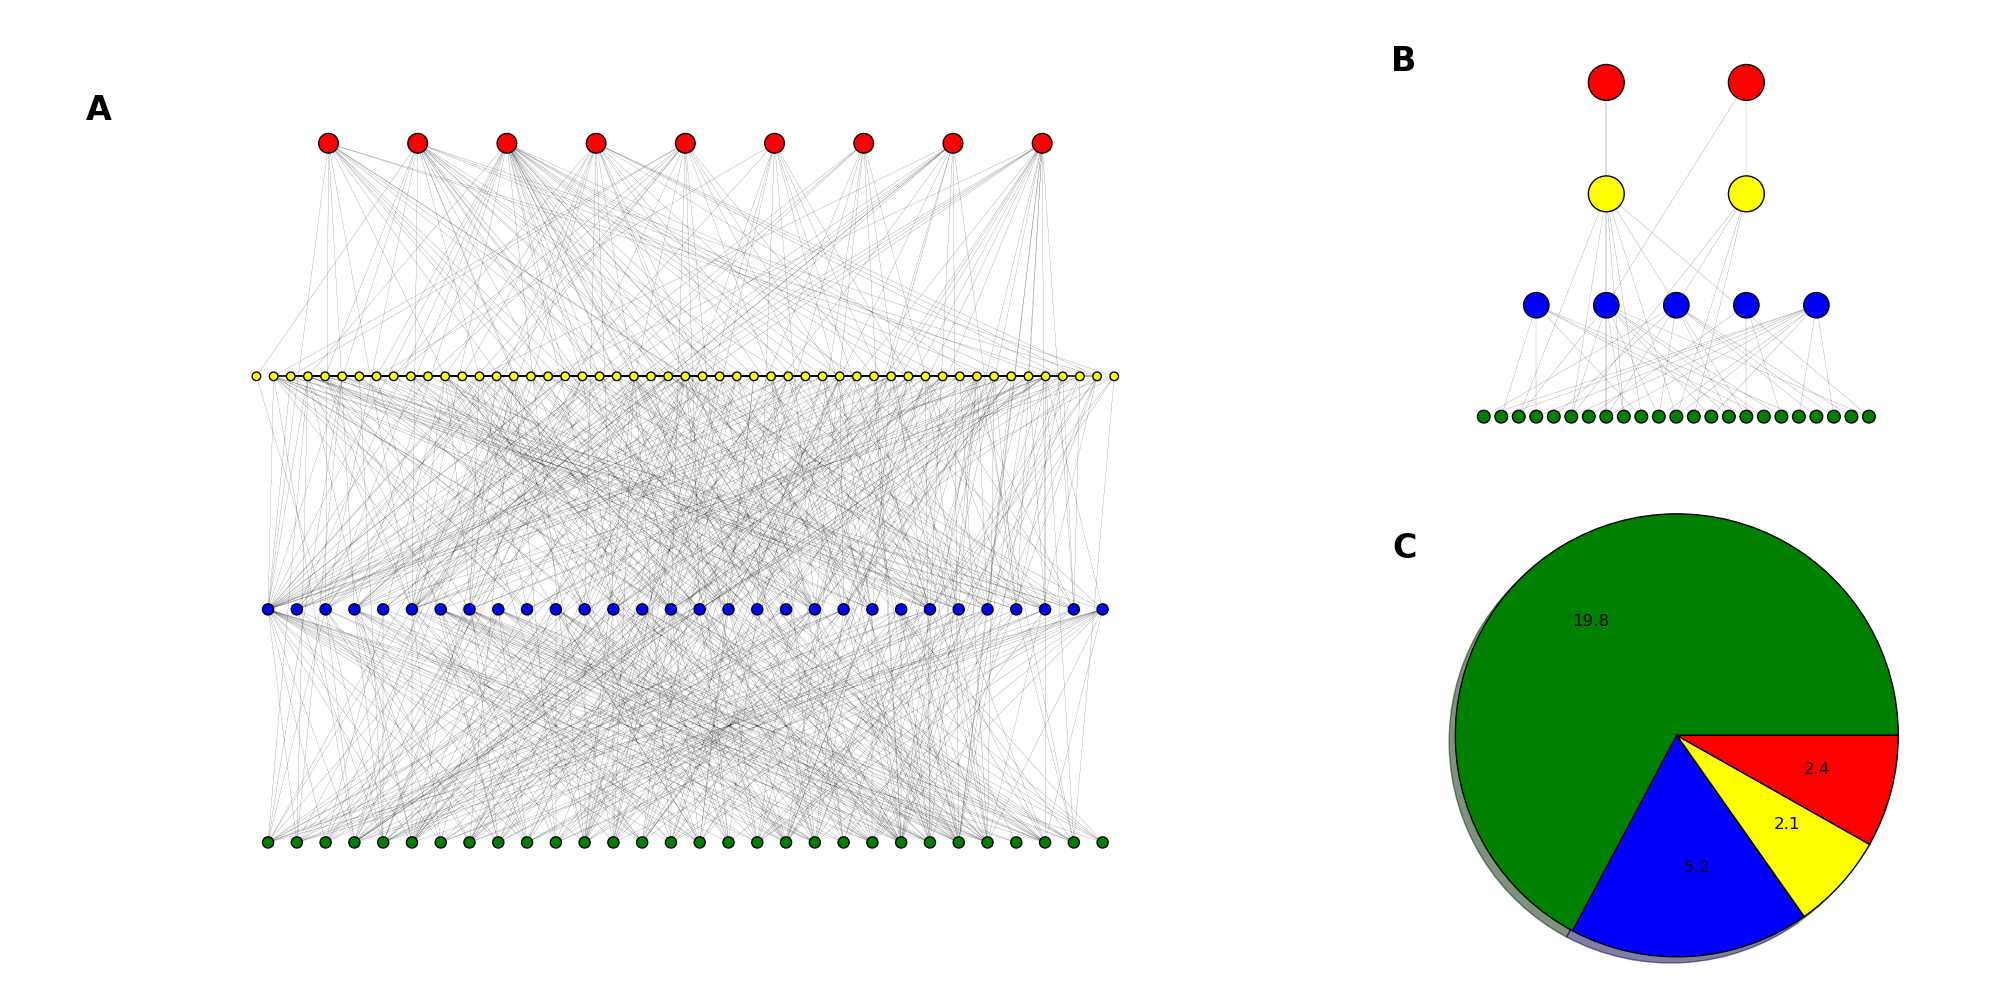
\includegraphics[width=\textwidth]{{{figures/persistence/net_struct/good_network_page}}}
	\caption{Example of a \textbf{`good network structure'.} Colours represent trophic level. (A) Antagonistic network of 120 species, rewired from the niche model. (B) Example of the `pruned' network consisting of species that persist after 5000 iterations. (C) Mean number of species belonging to each trophic level in the pruned network, averaged over 100 replicate simulations (all using A as the initial network).}
	\label{fig:good_net_example}
\end{figure}

\begin{figure}
	\centering
	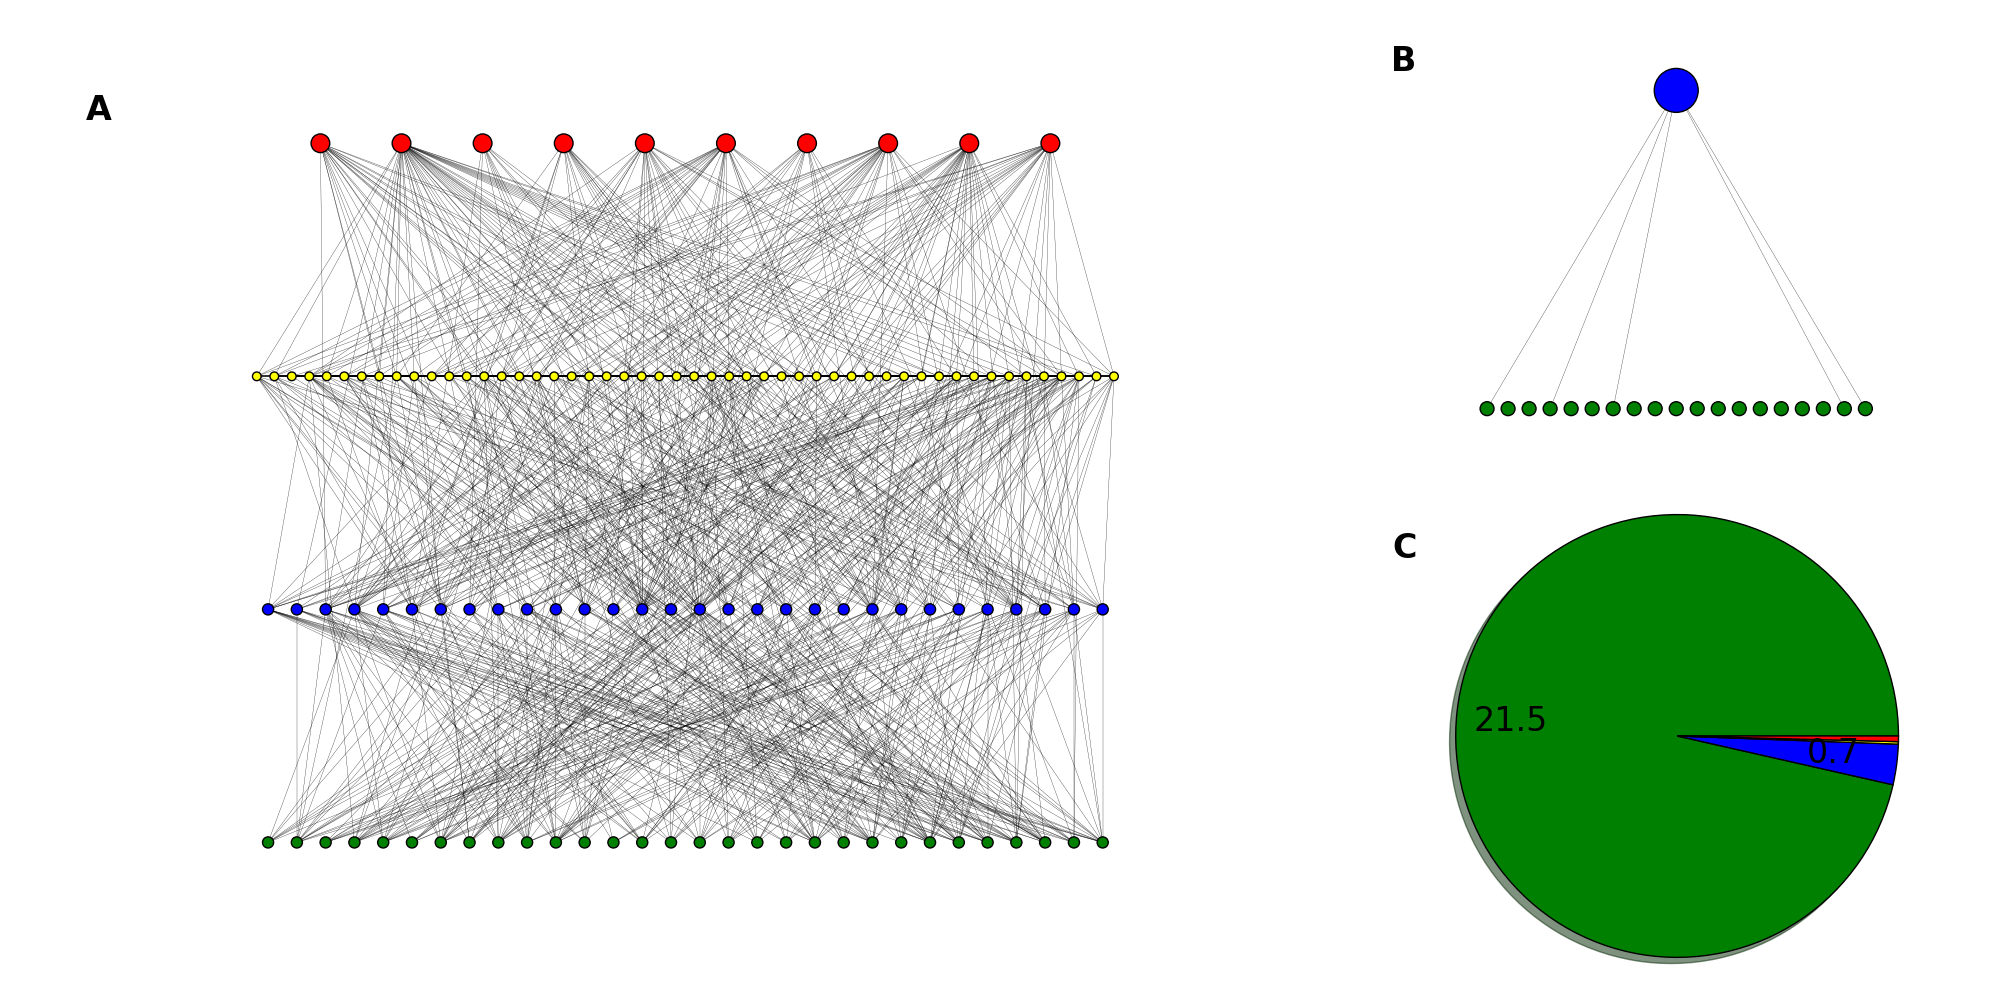
\includegraphics[width=\textwidth]{{{figures/persistence/net_struct/bad_network_page}}}
	\caption{Example of a \textbf{`bad network structure'.} Similar to figure \ref{fig:good_net_example}, but will a different initial network of 120 species.}
	\label{fig:bad_net_example}
\end{figure}
%
%\begin{figure}
%	\centering	
%	\renewcommand{\thesubfigure}{}
%	\setlength{\subfloatlabelskip}{0pt}
%	%\hspace{-2.5cm}
%	\subbottom[\textbf{Bad network}]{\includegraphics[width=0.8\linewidth]{"figures/persistence/temp/bad_network_rewired"}}
%	%\caption{The mean initial number of species belogning to each functional gropup.}
%	%\label{fig:trophic_dynamics_example}
%	\subbottom[\textbf{Good network}]{\includegraphics[width=0.8\linewidth]{"figures/persistence/temp/good_network_rewired"}}
%	\caption{Two 120 species interaction network. One produces better persistence than the other, although in both cases most species go extinct.}
%	\label{fig:good_bad_nets_120}
%\end{figure}
%
%\begin{figure}
%	\centering	
%	\renewcommand{\thesubfigure}{}
%	\setlength{\subfloatlabelskip}{0pt}
%	%\hspace{-2.5cm}
%	\subbottom[\textbf{Bad network}]{\includegraphics[width=0.8\linewidth]{"figures/persistence/temp/example_pruned_bad_network_rewired"}}
%	%\caption{The mean initial number of species belogning to each functional gropup.}
%	%\label{fig:trophic_dynamics_example}
%	\subbottom[\textbf{Good network}]{\includegraphics[width=0.8\linewidth]{"figures/persistence/temp/example_pruned_good_network_rewired"}}
%	\caption{Examples of the networks of species that remain at the end of a simualtion.}
%	\label{fig:good_bad_nets_pruned}
%\end{figure}



\subsection{Discussion}
\label{sec:disucss_persitence}

If the principle of \emph{competitive exclusion} holds, then that in such a situation the number of species will be less than or equal to the number of fundamental niches, or limiting resources: 
%http://onlinelibrary.wiley.com/doi/10.1046/j.1461-0248.2003.00551.x/full
But spatial patterns may reduce competitive exclusion?! - find a ref for this...but doesn't seem to happen in our model.

Since our species do not have traits that make differential use of resources we expect this number to be low..

Good/bad networks structure suggests interesting role of topology in defining the possible number of species...(have got refs on this)..but a more detailed investigation is beyond us..many topologies ot explore...(cite Thilo).

Importance of immigration in shaping real world communities. In our model it is essential!

It may be that there exists somewhere a region of stable coexistence of all species for zero IR. If there does, we will not find it. 


MAI ratio has small but detectable cascading effects on persistence and relative abundance in higher trophic levels. However the main benefit is to species that interact mutualistically. This may be a modelling issue and in nature it may well be that the cascading effects are stronger (or indeed opposite!)

Reproduction rate has a stronger cascading effect, improving RA and persistence in higher trophic levels. This is very realistic. HOwever in our model it still does not create proper biodviersity...

Landscaoe size has some small effect on persistence (mainly for plants?) - presumably due to reduced competition for space. Does not fix the problem.

Number of initial species 

Network structure: some networks are better than others. Further analysis could look at why this is (netowrk metrics). However we do not do this here because of the large number of topologies that would need to be explored (cite Thilo), and it is not relevant ot the main drive of the narrative. We did do a preliminary analysis of network metrics (generality, vulnerability, modularity - see previous chapter), but did not find any correlation between these and persistence. HOwever it does appear...more depth could reveal somethign interesting here..

Conclusion: immigration is required in our model to prevent competitive exclusion.  

MAIN POINT FOR FOLLOW ON: So we have a regime of high immigration (IR$=0.005$) where we see no extinctions under extreme habitat loss, and a regime of zero IR where we see many extinctions in pristine landscape. In between these two extreme must lie a region of interest where there are persistent and diverse communities at low levels of HL, which display extinctions for increasing levels of HL. We investigate this.


\clearpage
\section{Stationarity}
\label{sec:intro_stationarity}
%% Alternative titles: steady-state assumption? The problem with variability...

\begin{figure}
	\centering
	\includegraphics[width=0.8\textwidth]{"figures/stationarity/cov_vs_ir"}
	\caption{\textbf{Temporal variability} versus immigration rate (IR). Each points shows the mean value of the metric over 50 replicate communities, and the error bars show $\pm$ one standard deviation.}
	\label{fig:cov_vs_ir}
\end{figure}

As we began to investigate the region between zero immigration and high immigration rate we found a robust feature of the model - reducing immigration rates \emph{increases the temporal variability} of the dynamics. Here temporal variability is measured using the same metric described in chapter \ref{chap:habitat_loss_high_immigration}\footnote{Check that this is still where the metric is defined!}, i.e. the coefficient of variation in species population dynamics, averaged over all species in the community. In the previous chapter \emph{contiguous} habitat loss was shown to increase temporal variability, up to a average value of $\sim 0.3$ for HL$=90\%$\footnote{Reference figure in previous chapter?}. Figure \ref{fig:cov_vs_ir} illustrates that reducing the immigration rate can push the temporal variability well above this level, even in pristine landscape. 

This increased variability may bring into question the validity of results derived from the simulation output. Implicit in our analysis so far is the assumption that \emph{stationarity} (see section \ref{sec:stationarity}) is reached by the end of the simulation. The results presented in the previous chapter (and in \cite{lurgi2015effects}) are either calculated from a `snapshot' of the simulation state on the final (5000th) iteration or, in the case of the network and variability metrics, are calculated from samples aggregated over the final 200 iterations. For results obtained in this way to be reliable the simulation must reach a sufficiently steady state after 5000 iterations. In the high immigration regime (HIR) it may be reasonable to assume that this is the case. In the HIR simulations that we inspected the main transient dynamics are contained within the first 1000 iterations, which is followed by a period of relatively constant abundance (see for example figure \ref{fig:hi_trophic_dynamics})\footnote{Clearer: sampling from s steady-state distribution. Also this is How Lurgi et al do it}. However we are now motivated to investigate this steady-state assumption. In section \ref{sec:stationarity} we conduct a detailed analysis of the \emph{stationarity} of population dynamics generated by the IBM model. We then move on, in section \ref{sec:reliability}, to look at how our numerical results are affected by increased variability, and how this relates to the sampling regime. Finally we close the chapter (section \ref{sec:determinism}) by applying to test for determinism, to address the concern that the simulations may become dominated by randomness. In the discussion (section \ref{sec:discussion}) we justify the continued use of the model, and relate our findings to the debate on the stability and stationarity of real-world ecosystems\footnote{Make this better!}.
 
%However we are now motivated to investigate `how constant' the simulations are after the initial transience, and how this might affect our results.


\subsection{Second-order stationarity}
\label{sec:stationarity}
%\begin{itemize}


%	\item Justify choice of weak-stationarity
%	\item discuss tests for weak stationarity e.g. Nason \cite{ref:nason2013test}. PSR. ADF. KPSS. define them.
%	\item mention use of wavelets in ecological time series - reffer to PSR test 		
%	\item Choice of metric to look at : total number of individuals, or by species?? (justify both..)
%\end{itemize}

We introduce here three tests for second-order (or `weak') stationarity in time series.  Second-order stationarity may be defined as the time invariance of the first and second moments of the data. Specifically Hsu \cite{hsu1997schaum} states that a random process $X(t), t \in \mathbf{Z}^+$ is second-order stationary if:

\begin{eqnarray*}
	\mathbf{E}[X(t)] &=& \mu \text{ (constant),} \\
	R_X(t,s) &=& \mathbf{E}[X(t)X(s)] = R_X(|s-t|), 
\end{eqnarray*}

where $R_X(t,s)$ is the \emph{autocorrelation} function of the process. Conceptually these conditions state that a second-order stationary time series has constant mean and autocorrelation dependent only on time separation. From now on we will refer to this just as \emph{stationary}. If the conditions are not met we call the time series \emph{non-stationary}, and we cannot parameterise a constant distribution for the data. Non-stationarity may be due, for example, to a trend in the data or a change in the parameters of the data generator. 

In our case the data generator is the IBM model and there are several possible causes of non-stationarity. It may be that there is no steady-state equilibrium in the model. For example the number of individuals may undergo a random-walk. From previous analysis this situation seems unlikely, since we have observed what appear to be deterministic population cycles. However randomness has not been explicitly tested for. Another possibility is that a steady-state equilibrium exists, but that a long transience  means it is not reached during the time frame of our simulations.

%%Intuitively this is the definition of stationarity we are looking for in the model output - if the generated time series is weakly stationary then the simulation has reached a steady state distribution, and the results that we take involve sampling from this distribution. The repeatability of the results then only depends on the properties of this dsitribution (we also need to look at individual species..see later). 

\subsubsection{Tests for stationarity}
\label{sec:stat_tests}

We compare three different tests of stationarity: the Kwiatkowski-Phillips-Schmidt-Shin (KPSS) \cite{kwiatkowski1992testing}; the Augmented Dickey-Fuller (ADF) \cite{said1984testing}; and the the Priestley-Subba Rao (PSR) \cite{priestley1969test} tests. These tests were chosen for their popularity in the time series literature. All three are implemented in the programming language \emph{R} \cite{Rlanguage} - the former two in the package \emph{tseries}, and the latter in the package \emph{fractal}.

The ADF test has null hypothesis that the time series is non-stationary. The test models the data as an auto-regressive process (see section \ref{sec:stationarity_discussion}), and the null hypothesis is that this process has a \emph{unit root}. The test produces a statistic that is negative. The greater the magnitude of the test statistic the more evidence there is to reject the null hypothesis in favour of stationarity.

The KPSS test complements the ADF test in that the null hypothesis is stationarity. The data is modelled as the sum of a random-walk and an error component, and tests the hypothesis that the variance of the random walk is zero. The test statistic is always positive, and the greater its magnitude the more evidence there is to reject the null hypothesis in favour of non-stationarity.

The null hypothesis of the PSR test is also that the series is stationary. The test is based on the idea that non-stationary processes have power spectra that change over time \cite{priestley1969test}. These are called \emph{evolutionary spectra}. The test, as implemented in \emph{R}, returns several statistics. We quote the `p-value for T' which can be thought of as the confidence that the estimated spectral density functions are constant in time.

\subsubsection{Characterising the tests}
\label{sec:characterising_stat_tests}

%% metnion that time series must be one-D??

To understand the performance of the stationarity tests (section \ref{sec:stat_tests}) we apply them to three example time series, which we refer to as HI, RW and NS. The first series, HI, is taken from a single IBM simulation run with high immigration rate (IR$=0.001$), zero mutualism (MAI$=0.0$) and otherwise default parameters (table \ref{tab:whereis}).  The series represents the total number of individuals of all species at each iteration. The simulation was run for 50,000 iterations, compared with the 5000 used in previous chapters. The increased length allows more time for the simulation to reach stead-state, and allows comparison of tests applied to different sections of the series. The first 1000 iterations were discarded, since these contain clearly transient dynamics (see figure \ref{fig:hi_trophic_dynamics}B), leaving a time series of 49,000 points. A high immigration rate was chosen because it reduces the temporal variability of the dynamics, as was discussed in chapter \ref{chap:varying_immigration_rate}. Therefore the HI series is more likely to be stationary than the output of a simulation with a lower IR (section \ref{sec:ensemble}).

The series RW and NS are chosen as a negative and a positive control respectively. Both have the same length as HI. RW is a non-stationary series generated by a one-dimensional \emph{random-walk}, defined as:

\begin{equation}
	x(t) = \Sigma_{t}^{i=1} Z_i, 
\end{equation}   

where $Z_i$ are independent random variables that may take a value of either $-10$ or $+10$, both with probability half. An ensemble of such random walks was generated and a single instance was chosen with mean and variance closest to the HI series. RW has a mean and standard deviation of 15525.2 and 1549.8 respectively, compared to 15915.8 and 1545.6 for HI. For comparison, NS is a stationary series generated by drawing each value independently from a normal distribution with mean and variance  equal to that of HI. The three series are plotted in figure \ref{fig:adf}.
  
%We know that such a series is non-stationary in general (although it may appear stationary by chance?).
  
\begin{figure}[ht]
	\centering
	\includegraphics[width=0.8\linewidth]{"./chapters/chapter04b/figures/hi_rw_ns_dynamics"}
     \caption{The three time series used to characterise the performance of the stationarity tests. The intial 1000 points removed such that all are 49,000 points long. \textbf{(A) HI}: total abundance dynamics of an IBM simualtion with high immigration rate; \textbf{(B) RW}: a random walk without drift, as described in the text; and \textbf{(C) NS}: a series generated by independent sampling from a normal distribution.} 
     \label{fig:adf}   
\end{figure}

\begin{table}[h!]
\centering
\label{tab:adf_psr_kpss_whole}
\begin{tabular}{|
>{\columncolor[HTML]{C0C0C0}}c |c|
>{\columncolor[HTML]{9AFF99}}c |c|c|c|c|}
\hline
   & \multicolumn{2}{c|}{\cellcolor[HTML]{C0C0C0}A.D.F.}                 & \multicolumn{2}{c|}{\cellcolor[HTML]{C0C0C0}P.S.R.}              & \multicolumn{2}{c|}{\cellcolor[HTML]{C0C0C0}K.P.S.S.}                  \\ \hline
   & \cellcolor[HTML]{C0C0C0}stat & \cellcolor[HTML]{C0C0C0}p-value      & \cellcolor[HTML]{C0C0C0}stat & \cellcolor[HTML]{C0C0C0}p-value   & \cellcolor[HTML]{C0C0C0}stat & \cellcolor[HTML]{C0C0C0}p-value         \\ \hline
HI & -15.401                      & {\color[HTML]{333333} \textless0.01} & -                            & 0.0004782808                      & 0.5395                       & 0.03277                                 \\ \hline
RW & -4.0386                      & {\color[HTML]{333333} \textless0.01} & -                            & \cellcolor[HTML]{9AFF99}0.9929773 & 18.7453                      & \textless0.01                           \\ \hline
NS & -37.5348                     & {\color[HTML]{333333} \textless0.01} & -                            & \cellcolor[HTML]{9AFF99}0.811097  & 0.0466                       & \cellcolor[HTML]{9AFF99}\textgreater0.1 \\ \hline
\end{tabular}
\caption{Results of applying the three stationarity tests to the example time series shown in figure \ref{fig:adf}. P-values that indicate evidence for stationarity at $95\%$ confidence are highlighted in green. The test statistics are also given for the ADF and KPSS tests.}
\end{table}

Initially we apply the three stationarity tests to the entire length of the time series. The results are shown in table \ref{tab:adf_psr_kpss_whole}. ADF finds significant evidence that all three series are stationary, at $99\%$ confidence. We may be suspicious of this result since we know that RW is generated by a non-stationary process.  However this is a special case of a random walk, chosen from several thousand to closely match the mean and variance of HI. Therefore it may not be unreasonable that it can pass as stationary. The test statistic for ADF indicates that there is most evidence for NS to be stationary, followed by HI, then RW.
  The KPSS test ranks the series in the same order, based on the magnitude of the test statistic. According to this test NS is clearly stationary (accept h0), and RW is clearly non-stationary (reject h0 at $99\%$ confidence), whilst HI is borderline. For HI we would accept the null-hypothesis of stationarity at $95\%$ confidence, but reject it at $99\%$. 

The PSR test gives unexpected results. It concludes that RW and NS are both stationary, whilst HI is non-stationary with a high degree of confidence (p-value$<0.001$). In fact, according to PSR, RW is more likely to be stationary than NS. This result contradicts what we know about the series. Therefore we do not use this test in the analysis that follows. However the apparently erroneous result may contain interesting information about the HI series and the process that generated it (see discussion in section \ref{sec:stationarity_discussion}. 


%% WUOLD BE NICE BUT ANALYSIS NEEDS RE-DOING...
%\begin{figure}[hp]
%	\centering
%    \subbottom[Sample size = 1000 iterations]{\includegraphics[width=0.8\linewidth]{"./chapters/chapter04/figures/steadystate/hi_rw_ns_zscore_wl1000"}}
%    \subbottom[Sample size = 5000 iterations]{\includegraphics[width=0.8\linewidth]{"./chapters/chapter04/figures/steadystate/hi_rw_ns_zscore_wl5000"}}
%        \caption{The z-statistic used to test the null hypothesis that sample means are drawn from the stationary distribution. Each dot indicates a sample from the dynamics, which is tested.}    
%    \label{fig:zscore}
%\end{figure}


\begin{figure}[h!]
	\centering
	\includegraphics[width=0.80\linewidth]{"./chapters/chapter04b/figures/Rtests/stat_tests_v_wl"}
     \caption{Two tests for stationarity applied to samples of varying size (window length). Samples are taken from the three time series (HI,RW,NS) shown in figure \ref{fig:adf}. All three time series contain 49,000 points. Sample windows begin at the first point and increase in length from 1000 to 49,000 points. Points plotted at 0.01 indicate p-values less than or equal to this. (A) ADF test, with p-values capped at 0.20. 95th and 99th percentile in yellow and green respectively, indicating significant vidence for stationarity. (B) KPSS test, with p-values capped at 0.1. 95th and 99th percentile in orange and red respectively, indicating significant evidence for non-stationarity.} 
     \label{fig:stat_tests_v_wl}   
\end{figure}

Having discarded the PSR test, we now apply ADF and KPSS to samples of varying sizes, taken from the three series (HI,RW,NS). Sampling begins at the first point of the series and takes consecutive points up to the desired length of samples. Sample lengths range from 1000 to 49,000 data points. Again, as we saw in table \ref{tab:adf_psr_kpss_whole}, the two tests perform differently. The KPSS test correctly identifies RW and NS as non-stationary and stationary respectively, for all sample sizes. This is shown in figure \ref{fig:stat_tests_v_wl}B. The ADF test (figure \ref{fig:stat_tests_v_wl}A) correctly identifies NS as stationary for all sample sizes.  For short sample sizes it also correctly identifies RW as non-stationary. However, for sample sizes much above 20,000, ADF finds significant evidence that RW is stationary at $95\%$ confidence. This is an interesting result. Although RW is generated by a non-stationary process, it appears to fool the ADF test by staying `stationary enough' over many time points. 
  
There is mixed evidence for the stationarity of HI, as shown in figure \ref{fig:stat_tests_v_wl}. ADF, for all sample sizes above 2000, finds significant evidence that HI is stationary. Whereas KPSS, on the whole, gives significant evidence that HI is non-stationary - There are only seven cases where there is insufficient evidence to reject the null hypothesis that the HI series is stationary, and these occur at sample sizes between 24,000 and 34,000. From these results it appears that the KPSS test is a stricter test of stationarity, and is less sensitive to the size of the sample. Although it appears that the ADF test is biased in favour of stationarity, it does order the series correctly in the above examples and is a useful complement to KPSS. Also it may be that the sensitivity of ADF to sample length is useful, since processes may appear stationary/non-stationary at different scales. 

We consider the possibility that the method of sampling from the time series affects the results of the stationarity tests. For example samples taken near the beginning of an IBM simulation run may be more likely to give the non-stationary series because of transient dynamics. Alternatively a non-stationary data generator may produce sections of time series that appear stationary purely by chance. This sensitivtiy to sampling is investigated by \emph{reversing} the time series and repeating the above analysis. For HI, RW and NS we see no qualitative change in the results presented above. We also scan sampling windows of fixed length along the series to look for time dependence in the test results. The time at which samples are taken appears to make no qualitative difference, and there is no systematic change in the results that would suggest the simulation becomes more stationary the longer it is run\footnote{Note that this is not necessarily the case when we move to lower IRs.}. 


%% THINK THIS IS NOT NEED TO CHARACTERISE THE TESTS..MAYBE JUST DISCUSS IN THE TEXT?
%\begin{figure}[h!]
%	\centering
%	\includegraphics[width=0.8\linewidth]{"./chapters/chapter04b/figures/Rtests/stat_tests_v_time"}
%     \caption{Similar to figure \ref{fig:stat_tests_v_wl} but with samples of fixed sample size taken from different parts of the time series. To sample windows of given length (wl) are moved along the series and the tests are applied to the sub-series that falls within the window. Results are plotted against the mid-point of the window.}
%     \label{fig:stat_tests_v_time}   
%\end{figure}

\begin{figure}[h!]
	\centering
	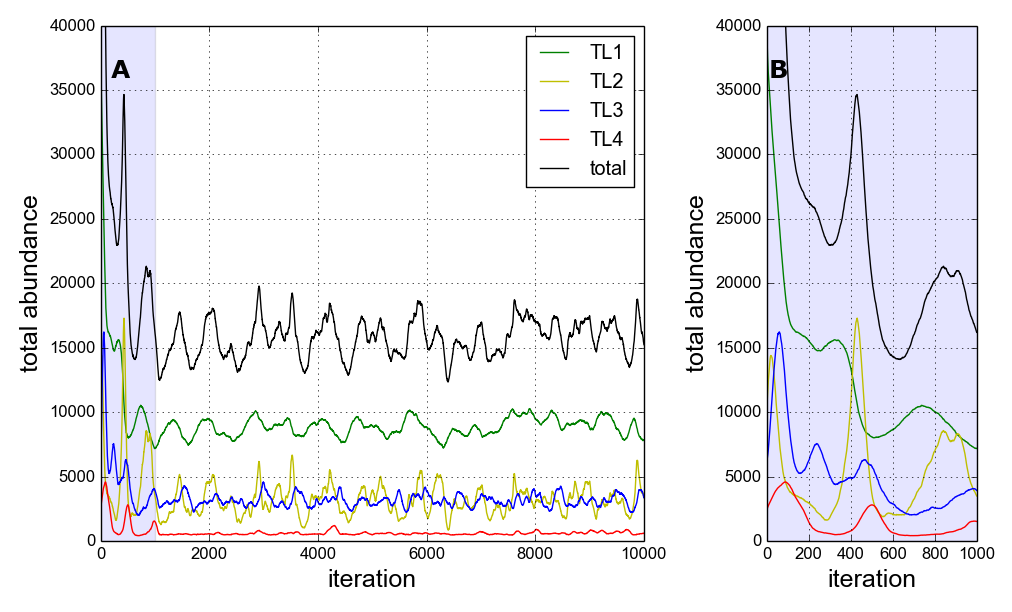
\includegraphics[width=0.7\linewidth]{{{figures/stationarity/hi_trophic_dynamics}}}
     \caption{Dynamics for the HI simulation, broken down by trophic level ($TL1-4$). Abundance is measured by the number of individuals. (A) Part of simulation run (total = 50,000 iterations). (B) Enlaregement of first 1000 iterations, showing transience.} 
     \label{fig:hi_trophic_dynamics}   
\end{figure}


\paragraph*{HI simulation.}
We now focus on the simulation data used to generate HI and look in more depth at whether this dataset can be considered stationary. We use the same two tests, ADF and KPSS, for the stationarity of univariate time series. Since our abundance vector is 60-dimensional ($N=60$ species), it is necessary to perform some manipulation to get a time series we can test. Previously we used the total number of individuals as our time series. However simply summing over species (l1-norm) is not necessarily the most informative metric to use. One possible issue is that the phase differences between species oscillations that we would expect due to trophic interactions (see chapter \ref{chap:whereis}) may mean that temporal variability is cancelled out when aggregating abundances in this way. It is possible that simulations which appear stationary according to some aggregate metric (e.g. total number of species) may have non-stationary underlying dynamics. This suggests that it is most informative to consider stationartiy at the species level. We also consider the stationarity of abundances by trophic level, as an alternative aggregate metric.

The dynamics of the HI simulation are aggregated by trophic level to create four new time series TL$1-4$. These \emph{trophic dynamics} are plotted in figure \ref{fig:hi_trophic_dynamics}. The initial period of transience is expanded in panel B. As in the previous analysis this part of the time series (first 1000 iterations) is removed. The ADF and KPSS tests are applied to the four trophic series separately and the results are shown in figure \ref{fig:tl_stat_tests_v_wl}. According to ADF all trophic levels are stationary for samples sizes greater than 4000. TL1 appears to be least stationary according to ADF, requiring a sample size of at least 4000 before to reject the null hypothesis at $95\%$ confidence. According to KPSS TL1 is non-stationary for all sample sizes, whilst TL2 and 3 are stationary for samples sizes above 6000 and 1000 respectively. KPSS gives mixed results for TL4, with no clear dependnence on sample size. It is hard to reconcile these results with an observation of the dynamics in figure \ref{fig:hi_trophic_dynamics}, indicating the usefulness of the statistical tests. It may be informative to consider if there are general trends in the stationarity of trophic levels.

\begin{figure}[h!]
	\centering
	\includegraphics[width=0.8\linewidth]{"./chapters/chapter04b/figures/Rtests/tl_stat_tests_v_wl"}
     \caption{Similar to figure \ref{fig:stat_tests_v_wl}, but here the tests are applied separately to each trophic level of the HI simulation. The four time series (TL$1-4$) represent the total number of individuals belonging to each trophic level at every iteration.} 
     \label{fig:tl_stat_tests_v_wl}   
\end{figure}

The dynamics of all the species belonging to each trophic level are plotted in figure \ref{fig:dynamics_by_species}. It is clear here that the community is dominated by a few abundant species, mainly in the lower trophic levels, with a large number of relatively scarce species. This is agrees with the rank abundance plots from chapters \ref{sec:whereis}, and with the long tailed distributions seen in real world communities. It also appears from this figure that the more abundant species exhibit large amplitude oscillations in their dynamics. This leads us to hypothesise that the most abundant species may be non-stationary, whereas the least abundant species may be stationary. We test this hypothesis by applying the ADF and KPSS tests to the three most abundant and three least abundant species in the HI simulation. Species are selected based on their average abundances over the whole simulation (minus the intial transience).  

\begin{figure}[ht!]
	\centering
	\includegraphics[width=1.0\linewidth]{"./chapters/chapter04b/figures/hi_sp_by_tl_part10000"}
    \caption{Dynamics of every species in the first 10,000 iterations of the HI simulation, broken down by trophic level. Panels (A)-(D) show all the species belonging to each trophic level (TL$1-4$).}    
    \label{fig:dynamics_by_species}
\end{figure}

We see from figure \ref{fig:sp_stat_tests_v_wl} that all six species are stationary according to ADF, given sufficiently large sample size. However the sample size for all three of the abundant species to be stationary is greater (panel A: $\geq 9,000$ points) than for the three least abundant species (panel C: $\geq 2,000$ points). This suggests that the most abundant species are indeed `less stationary' than the least abundant species. The KPSS test supports this conclusion. KPSS finds that the three least abundant species are stationary above samples sizes of $\sim 18,000$, whereas two of the most abundant species are non-stationary for almost all sample sizes. Inspecting the dynamics in figure \ref{fig:dynamics_by_species} we see that these non-stationary species are those with largest amplitude fluctuations in their abundances. 

In general we conclude that the choice of metric used to generate the time series does affect the conclusions about stationarity. Overall we cannot be confident that the HI simulation is stationary, based on the results presented above for species, trophic and total abundances. This is largely due to the apparent strictness of the KPSS test. Considering species dynamics individually is the most informative. It allows for the possibility that some species abundances may be more variable than others, and information is not lost by aggregating.  In the following analysis we propose that stationarity tests should be applied to species dynamics, and then the number of stationary species (NSSP) used as an aggregate statistic. If NSSP equals the total number of species, then the community dynamics is fully stationary (according to the test used).   

%\begin{figure}[hp]
%	\centering
%    \subbottom[Sample size = 1000 iterations]{\includegraphics[width=0.8\linewidth]{"./chapters/chapter04b/figures/hi_sp_by_tl"}}
%    \subbottom[Sample size = 5000 iterations]{\includegraphics[width=0.8\linewidth]{"./chapters/chapter04b/figures/hi_sp_by_tl_part10000"}}
%        \caption{The dynamics of individual species.}    
%    \label{fig:dynamics_by_species}
%\end{figure}

\begin{figure}[hp]
	\centering
	\subbottom[Three most abundant species]{\includegraphics[width=0.8\linewidth]{"./chapters/chapter04b/figures/Rtests/sp_ma_stat_tests_v_wl"}}
		\subbottom[Three least abundant species]{\includegraphics[width=0.8\linewidth]{"./chapters/chapter04b/figures/Rtests/sp_la_stat_tests_v_wl"}}
     \caption{Similar to figure \ref{fig:stat_tests_v_wl}, but here the tests are applied separately to individual species from the HI simulation. (A) The abundance time series of three species with highest average abundances. (B) The three species with lowest average abundance.} 
     \label{fig:sp_stat_tests_v_wl}   
\end{figure}

\newpage
\subsubsection{Stationarity results}
\label{sec:ensemble}

We now pursue a general investigation of the stationarity of communities simulated with the IBM model. First we test the stationarity of three ensembles of new simulation runs (figure \ref{fig:hi_v_li_net7_ensemble}). Secondly we test the simulations used to generate the results presented in the previous chapter (figures \ref{fig:nssp_ir_v_hl},\ref{fig:nssp_v_ir_and_hl}). The new simulations use default parameters, unless otherwise specified, and are run for 50,000 iterations. Two ensembles of 100 simulations each are run for high (IR$=0.001$) and low (IR$=0.0001$) immigration rates, which we refer to here as the HI and LI ensembles respectively. A third ensemble of 50 shorter simulations (10,000 iterations) is run, at high immigration rate, using a fixed interaction network, which we call the NM1 ensemble. All networks are generated using the niche model as described in section \ref{sec:whereis}, with zero mutualism (MAI=$0.0$). Each simulation uses a uniquely generated network, except for those of the NM1 ensemble. Stationarity testing is done using the ADF and KPSS tests characterised in section \ref{sec:characterising_stat_tests} above. As standard the initial 1000 iterations are discarded in an attempt to remove transience. The tests are then applied to a sample taken from the abundance time series of each species. The results presented in this section give the number of stationary species (NSSP) in the community, at the $95\%$ confidence level.

As the length of the samples taken from the abundance time series increases, the average NSSP also increases. This is true of both tests and for all three ensembles, as we can see from figure \ref{fig:hi_v_li_net7_ensemble}A. According to ADF all species are stationary, on average, for sufficiently large sample length. The required length of sample is larger for the LI ensemble than for HI. For KPSS, although the NSSP does increase with sample length, it is not clear that it will asymptotically approach 60 species in the limit of many iterations. The average NSSP at 49,000 sample points is just under 40 and   just over 20 for HI and LI ensembles respectively.

To check the time dependence of stationarity (i.e. are species more likely to be stationary after many iteration of a simulation?) samples of length 3000 were taken from different points along the time series. From figure \ref{fig:hi_v_li_net7_ensemble}B we can see that there is no clear trend in in stationarity over 49,000 iterations. The average NSSP is almost the same whether the sample is taken from iterations 1000-3000 or 46,000-49,000. This result also holds for windows of different length, which are not plotted here.

On average we see that the LI ensemble is less stationary than the HI ensemble. This we expected from the results of chapter \ref{chap:whereis}. However we cannot be confident that either ensemble contains communities with stationary species distributions. This may be problematic for the interpretation of our results, and we discuss this further below. Interestingly the NM1 ensemble gives very similar results to the HI ensemble. This may be because we have accidentally chosen NM1 to closely resemble the average of this ensemble (see both panels of figure \ref{fig:hi_v_li_net7_ensemble}. Alternatively it may be that stationarity of the simulation output is not dependent on the interaction network structure. Again, we will return to this issue in what follows.

\begin{figure}[h]
	\centering
	\includegraphics[width=1.0\linewidth]{"./chapters/chapter04b/figures/hi_v_li_net7_ensemble"}
    \caption{The number of stationary species (NSSP) according to the two stationarity tests (ADF and KPSS), averaged over three different ensembles of simulations: HI(ensemble); HI(NM1) and LI(ensemble)  as described in the text. The first two are high immigration runs, whilst the latter is low immigration. Solid lines indicate the mean results for the ensemble, and error bars indicate $\pm 1$ standard deviation from the mean. (A) Each species abundance time series is sampled with a window of increasing length, as in figure \ref{fig:sp_stat_tests_v_wl}. (B) Each species series is sampled with a window of length wl=$3000$, which is scanned along the series as in figure \ref{fig:stat_tests_v_time}. For both tests results are interpretted at the $95\%$ confidence level.}    
    \label{fig:hi_v_li_net7_ensemble}
\end{figure}

\paragraph*{Previous simulations.} The simulations from chapter \ref{chap:wehereis} are tested for stationarity. All simulations are 5000 iterations long. The initial 1000 iterations are discarded and the ADF and KPSS tests applied, species by species, to the remaining 4000. Figure \ref{fig:nssp_ir_v_hl} shows the average NSSP across the region of parameter space investigated, for three MAI ratios (MAI$=0.0,0.5,1.0$). The results are qualitatively the same for both tests, although NSSP is higher for ADF than for KPSS as expected. On average reducing IR reduces the NSSP. A weaker effect, but still visible is that increasing HL reduces the NSSP. Most striking is the effect of MAI ratio on stationarity - the average NSSP is greater across the whole parameter region at MAI$=0.0$ than at MAI$=1.0$, with MAI=$0.5$ in between the two. Increasing mutualism also appears to reduce the dependence of NSSP on IR.  Figure \ref{fig:nssp_v_ir_and_hl} summarises these trends using cross sections taken from the heat maps in figure \ref{fig:nssp_ir_v_hl}, with error bars added. It is clear that there is high variability across replicate simulations, and this variability appears to be greatest for high mutualism (MAI=$1.0$).

\begin{figure}[hp]
	\centering
	\includegraphics[width=1.0\linewidth]{"./chapters/chapter04b/figures/nssp_ir_v_hl"}
    \caption{The average number of stationary species (NSSP) according to the two stationarity tests (ADF and KPSS), across the slice of parameter space explored in chapter \ref{chap:whereis}. All simulations are 5000 iterations. Tests are applied to final 4000 iterations.}    
    \label{fig:nssp_ir_v_hl}
\end{figure}



\begin{figure}[h!]
	\centering
	\includegraphics[width=0.8\linewidth]{"./chapters/chapter04b/figures/nssp_v_ir_and_hl"}
    \caption{The number of stationary species (NSSP) according to the ADF test. The points show mean numbers and error bars show $\pm$ one standard deviation. Tests are performed on the same simulations depicted in figure \ref{fig:nssp_ir_v_hl}. (A) Plotted against immigration rate (IR), with zero habitat destruction. (B) Plotted against habitat destruction, with IR$=0.001$. }    
    \label{fig:nssp_v_ir_and_hl}
\end{figure}

\subsubsection{Discussion (`skeleton')}
\label{sec:stationarity_discussion}

(From here on the document is not complete. This discussion skeleton synthesises the ideas about stationarity, before the narrative turns to look at how results are affected by temporal variability (section \ref{sec:reliability}), and then to test for determinism and chaos (section \ref{sec:determinism}).)

Main conclusion: communities not guaranteed stationary, even in high immigration regime. Most important question - how does this affect our results?  Second most important question: why are they not stationary? Hypothesis: deterministic chaos? Alternative hypothesis: stochastic fluctuations about a stable equilibrium (but is this deterministic? and why would this not appear stationary?)

Importantly there is no evidence that the simulations are getting more stationary as they go on (i.e. 5000 iterations is probably enough) This means we do not need to throw away all previous results. But may need to reconsider how to calculate them.

%If not already done, talk about relative abundances of species and if these change due to oscillations..

Also to discuss:
\begin{itemize}
	\item Stationarity in real world communities (plankton, and look for more examples). Thermodynamics. Far from equilibrium systems.
	\item Other possible tests for stationarity (parametric vs non-parametric, are the tests we used OK??)
	\item PSR test: time dependent frequency spectra, possible use of wavelets (signature of aperiodic dynamics??)
\end{itemize}


The topic of this chapter is also relevant to our understanding of `real world' communities. The assumption that an ecosystem is in a \emph{steady-state} has often been often made \cite{brock1967ecosystem}. It is clear that ecosystems are dynamic, but they are remarkably robust and persistent in the face of environmental variability. For those who approach ecological theory from a dynamical systems perspective these properties are related to the dynamic stability of the system. Indeed to model an ecosystem as a dynamical system presupposes the existence of a stable equilibrium or attractor - otherwise the model could not explain observed species persistence. However it is not clear how to relate the concept of dynamic stability to the temporal variability of population dynamics, which is frequently used as a proxy for stability (there is an interesting and in depth treatment of this issue in \cite{arnoldi2015}). In an extreme example there may exist a chaotic attractor, which is highly stable but which creates highly variable population dynamics. In such a case the steady-state assumption does not seem appropriate. 


%Also discuss parametric tests and frequncy spectra:
%
%The first two tests (ADF and KPSS) makes assumptions about the process that generated the data. For example, in the case of the ADF test, it is assumed that the data can be modelled as an autoregressive process. Grazzini \cite{grazzini2012analysis} refers to such tests as \emph{parametric} and points out that their simple assumptions about the data generator process may be too restrictive (REPHRASE) for time series generated by complex systems models, such as our IBM.  With this in mind we proceed with these tests because they are part of the standard set of tools currently used for time series analysis. Interestingly the PSR test and another, test proposed by Nason \cite{nason2013test} and based on wavelets analysis of the time varying power spectrum, do not reuqire such parameteric assumptions...waveletts..waveletss..
%
%Regarding the PSR test - The test attempts to detect a time-varying power spectrum, as a signature of non-stationarity. This signature may be characteristic of adaptive dynamical systems, or systems exhibiting some kind of aperiodic dynamics. In general wavelets have proven a useful tool to study signals with time-dependent frequency spectra, and have found application in the analysis of non-stationary ecological time series \cite{cazelles2008wavelet, nason2013test}. However a preliminary investigation using the \emph{R} package \emph{biwavelet} did not appear fruitful and is not pursued further in this thesis\footnote{Although we may well refer back to this if we do discover chaos in the IBM!}. 





\subsection{Reliability of results}
\label{sec:reliability}

%The previous results from this chapter indicate that the simulated dynamics may be highly variable, with a deterministic and stochastic component dependant upon the parameters. Here we consider how this temporal variability affects our results. In particular we look at how sensitive measurements of abundance are to the length of sample taken from the dynamics\footnote{If we can be confident in our measurements of abundance we may be confident in other results also}. 

In chapter \ref{chap:habitat_loss_high_immigration} we used  `snapshots' of the simulation state to calculate species abundances. Clearly this sampling method yields different results depending on when the measurement is taken. The snapshot method was justified by the assumption that simulations reached stationarity and therefore we were sampling from a steady-state distribution (with suitably low variance). However, as we saw in section \ref{sec:intro_stationarity}, stationarity cannot be guaranteed. The results of section \ref{sec:determinism} suggest that this lack of stationarity is due to deterministic population dynamics, especially those of the most abundant species. Irrespective of the cause, here we look at how temporal variability affects the our results. In particular we focus on measurements of species abundance and how these depend on the length of sample taken from the dynamics. To do this we make the assumption that the \emph{long term average} abundance is what we want to measure.

\subsubsection{Abundances}

This analysis uses two metrics, both of which require the hypothesis that each species has an equilibirum abundance or long-term average abundance, which is well approximated by the mean abundance between 1000 and 50,000 iteration in the long simulations. (This is related to the idea of repeatability, which we look at below - is this long term average the same...RAS etc. for NM1)

Ideally we need to look at HI ensemble for IR=0.005 to justify original `snapshot' sampling - ask Alan.\\
**Need a plot to show how MRE is calculated..

%% These plots are a bit crap - how to improve?
%% Plotted using: habitat_loss_project/python_analysis_scripts/steady_state/test_files/lowIM/plot_averaged_species.py
\begin{figure}[hp]
	\centering
	\renewcommand{\thesubfigure}{}% no subfigure number
	\subbottom[\textbf{Raw dynamics}]{\includegraphics[width=1.0\linewidth]{"./chapters/chapter04b/figures/Reliability/LI/most_and_least_abun_species_dynamics"}}
	\subbottom[\textbf{Moving average filter (length=4000)}]{\includegraphics[width=1.0\linewidth]{"./chapters/chapter04b/figures/Reliability/LI/most_and_least_abun_species_dynamics_maf_wl4000"}}
		
    \caption{Example dynamics of (A) the most abundant and (B) the least abundant species, taken from a single simulation in the LI ensemble. Top: Raw dynamics (without averaging). Bottom: Moving average filter of length 4000 iterations. Dashed lines indicate the long term average throughout the whole simulation.}    
    \label{fig:maf_example}
\end{figure}

\begin{figure}[hp]
	\centering
	\subbottom[HI ensemble]{\includegraphics[width=1.0\linewidth]{"./chapters/chapter04b/figures/Reliability/LI/three_estimator_regression"}}
	\subbottom[LI ensemble]{\includegraphics[width=1.0\linewidth]{"./chapters/chapter04b/figures/Reliability/HI/three_estimator_regression"}}    
    \caption{Example of linear regression with the three estimators.}    
    \label{fig:regression_exmaple}
\end{figure}

\begin{figure}[h]
	\centering
	\includegraphics[width=1.0\linewidth]{"./chapters/chapter04b/figures/Reliability/error_versus_estimator"}
    \caption{Abundance estimator performance - use this to justify the way we take our measurements from simulations! The first estimator is a `snapshot' at 5000th iteration, the rest are averages of windows ranging from legnth 1000 to 50,000 in steps of 1000.}    
    \label{fig:error_versus_estimator}
\end{figure}

In this section we look at how reliable results are, how sensitive they are to different ways of measuring, and different lengths of averaging. 

At the end of the section we also look at repeatability using the ensemble NM1. And introduce RAS spectra.

\subsubsection{Variability: CoV}

Here we look at the CoV - how does it depends on the length of window used? 200 was used initially..

We may also look at CoV (or stationarity again) versus mean species abundance - do the more abundant species have higher temporal variability?

\subsubsection{Repeatability}

<<<<<<< HEAD
\begin{figure}[hp]
	\centering
	\includegraphics[width=1.0\linewidth]{"./chapters/chapter04b/figures/ras_3examples"}
    \caption{Rank abundance spectra (RAS) for three simulations run using the interaction network NM1 (see text). Species abundances are measured by taking the mean abundance over the final 1000 iterations of the simulation. The species are ranked according to their abundances in the first simulation (panel (A)). This odering is retained in panels (B) and (C), which represent different simulations. Colouring of species by trophic level is consistent with previous figures.}    
    \label{fig:ras_3examples}
\end{figure}


Repeats communites - do they always do the same things...NM1
=======
Repeat communities (simulate with same interaction networks) - do they always do the same things...NM1
>>>>>>> 205e25b4ac2e2d84c24bee8ea4a528f60ad29aaa

\begin{figure}[h!]
	\centering
	\includegraphics[width=1.0\linewidth]{"./chapters/chapter04b/figures/ras_dist"}
    \caption{The average rank abundace spectrum (RAS) for the ensemble of 50 simulations run using interaction network NM1 (see text). Species abundances measured as in figure \ref{fig:ras_3examples}, and ranked as in panel (A) of that figure. The main bars indicate mean abundance values, whilst the error bars indicate the minimum and maximum abundances over the ensemble.}    
    \label{fig:ras_dist}
\end{figure}

\clearpage
\subsection{Determinism tests}
\label{sec:determinism}

It is clear from the results in this chapter that population dynamics becomes highly variable, especially at low IR. From inspection of the population dynamics it appears that there is a strong stochastic component, even in the case of high immigration (for example Figure \ref{fig:dynamics_by_species}). This leads us to speculate that in some instances the simulation output may become dominated by randomness. This randomness is an interesting feature of the model, and indeed is likely to play an important role in real ecosystems (see discussion \ref{sec:discussion}). However much of our analysis (chapters \ref{chap:habitat_loss_high_immigration} and \ref{chap:varying_immigration_rate}) involves interpreting the simulation results in terms of the ecological mechanisms built into the model, in particular the patterns and structures generated by species interactions. If the model output lacks determinism it does not seem meaningful to conduct such analyses. Therefore we present here a test for determinism based on \emph{recurrence quantification analysis} (section \ref{sec:rqa}), which we then apply to our model output (section \ref{sec:rqa_results}).

\subsubsection{Recurrence quantification analysis}
\label{sec:rqa}      

Recurrence quantification analysis (RQA) maybe be used to detect signatures of determinism \cite{marwan2007recurrence,aparicio2008detecting,saul09phd}. The analysis is based on the idea of \emph{recurrence} - deterministic dynamical systems tend to return to similar regions of phase space. Moreover, when they do, their trajectories tend to remain close in phase space for some amount of time. In the case of chaotic systems the trajectories will diverge, at a rate which is broadly determined by the maximal Lyapunov exponent \cite{saul09phd}. However, even for chaotic systems, there is some tendency for neighbouring trajectories to remain close. RQA aims to detect the presence of this feature in the dynamics. The analysis is often used with univariate time series (such as in \cite{saul09phd}), in which case time-delay embedding must be used to increase the dimensionality of the phase space. However, since we have a time series for each of the 60 species, our phase space is already high dimensional. Therefore our first step is to construct a recurrence matrix (RM). The RM is a binary matrix whose elements, for a system $x(t) \in \mathbb{R}^N$, are given by the function:

\begin{equation}
d_{ij} = \begin{cases} 1 &\mbox{if } ||x(i)-x(j)||<r \\
0 & \mbox{if } ||x(i)-x(j)|| \geq r \end{cases},
\label{eq:rm}
\end{equation}
%
where $r$ is a threshold distance that defines the measure of `closeness' in phase space. Various methods have been proposed to choose the value of $r$. These methods are discussed in \cite{aparicio2008detecting}, but we use the method which they employ throughout their paper: $r$ is chosen such that $\sim 10\%$ of the elements of the RM are equal to one.

Having constructed the RM it can be visualised as a \emph{recurrence plot} (Figure \ref{fig:rec_plot}). Such plots can be visually striking (search recurrence plots for examples), but are difficult to interpret without experience. An important feature, in the search for determinism, are \emph{diagonal lines} - lines parallel to the leading diagonal. Such lines indicate that trajectories which find themselves `close' in phase space remain close, for a period of time given by the length of the line. Visual inspection can detect the presence of diagonal lines but it is better to use a quantitative pattern detection method. A common metric that quantifies the relative abundance of diagonal lines is the \emph{percentage of determinism} ($\%$DET) \cite{aparicio2008detecting,marwan2007recurrence}, and is given by:

\begin{equation}
\%DET = \frac{NPD}{NREC} \times 100,
\label{eq:pd}
\end{equation}
%
where NREC is the number of entries in the RM equal to one; and NPD is the total number of points found on diagonal lines of length greater than or equal to two. The $\%$DET allows quantitative comparison of the level of determinism between different RMs. In \cite{aparicio2008detecting} they develop three statistical tests, based on $\%$DET and two similar metrics, for the null hypothesis of pure randomness in the time series. However in the current analysis we make do with a comparison of the value of $\%$DET between different test cases.  

%Statistical tests can then be used to determine if the presence of diagonal lines is significantly greater than would be expected from a random time series. Three such test are presented in \cite{aparicio2008detecting}. Here we implement one of them, based on the metric they call \emph{average line length} (ALL).

%ARE WE GOING TO USE AVERAGE LINE LENGTH? WAIT AND SEE RESULTS BEFORE WRITING THIS UP. (may be better to just use $\%$det?) 

Mention sampling for speed! 

\subsubsection{Results}
\label{sec:rqa_results}

We test for determinism in the simulation ensembles HI and LI used in section \ref{sec:stationarity} (see for example Figure \ref{fig:hi_v_li_net7_ensemble}).  Each ensemble consists of 100 repeat simulations with different network structures. These simulations are used because one ensemble is from the high immigration regime (HI: IR$=0.001$) and one is from the low immigration regime (LI: IR$=0.0001$). Therefore the temporal variability is higher on average in the LI ensemble than the HI ensemble. The simulations in these ensembles are also longer than other simulations - being run for 50,000 iterations they allow for more chance of recurrent dynamics and therefore provide more information from which to detect a signature of determinism. In both ensemble the communities are antagonistic (MAI$=0$) and the landscape is pristine (HL$=0$). Therefore we do not cover the full range of parameters explored in other analyses, but we at least consider one highly variable and one less variable scenario.

For comparison of the values $\%$DET we construct randomised data in two different ways. In \cite{aparicio2008detecting} they state a random process would generate a RM with NREC points distributed uniformly at random\footnote{They actually say arbitrarily at random, but `uniformly' is better?}. We construct such matrices by randomly permuting the elements of another RM, to obtain a randomised RM with the same number (NREC) of points. In addition we also construct RMs by randomising the time series of each species. This preserves the mean and variance of the population dynamics, but removes any determinism. The randomised time series are then used to construct an RM\footnote{This description needs improving}.         

Figure \ref{fig:rec_plot} shows four example recurrence plots. Panels A and B show the RMs of single simulations from ensembles HI and LI respectively. Panels C and D show randomised versions of panel B generated by randomising the matrix, and by randomising the time series respectively. Panels A and B clearly have some structure, whilst the structure is lost in panel C as expected. Panel D retains some structure. In particular it contains the leading diagonal, since even the randomised time series is identically equal to itself. It also contains horizontal and vertical bands, created by points in the time close that are unusually distant (or close) to a large number of other points in the phase space. A subtle but detectable feature of panels A and B is the presence of diagonal lines (parallel to the leading diagonal) suggesting determinism. This feature is lost in panel D, as we would expected from the randomised time series. Interestingly panel A looks very similar to figure 1(c) in \cite{aparicio2008detecting}: an RM generated from the dynamics of a noisy chaotic Henon attractor (see discussion \ref{sec:discussion}).  

We calculate the $\%$DET for each simulation in the HI and LI ensemble. In each case, for comparison, we also calculate the $\%$DET for the dynamics of the ten most and ten least abundant species\footnote{Justify this, above?}, and for the two randomised versions of the data. These results are shown in figure \ref{fig:percentage_detemrinism}. The randomised data shows little variation, with a $\%$DET$\sim = 10$ in all cases.  The $\%$DET for the least abundant species is slightly greater than for random data, suggesting some evidence of determinism but also a strong stochastic component. In both the HI and LI ensembles there is good evidence for determinism at the whole community level, with $\%$DET consistently $>30$ and $>40$ respectively. It is interesting that there is more evidence of determinism in the LI ensemble than in the HI ensemble, as we were previously conserved that the high temporal variability of the LI dynamics could mean that it lacked determinism. It is also clear for these results that the deterministic component of the dynamics is dominated by the most abundant species. This, together with the results from previous sections tells us a lot about the dynamics of the model (see discussion below). We conclude here that the anlaysis so far suggests that non-stationarity may be largely due to to deterministic population dynamics/oscillations of the most abundant species, while the dynamics of the less abundant species are more random and more stationary although they appear to have a deterministic component.  

 
%Chaos - Although in many cases a statistical steady-state appears to be reached, there are complex dynamics and fluctuations within that state (see section \ref{whereis}).  Here we look at if these are due to noise or deterministic dynamics. We follow work presented by Saul in his PhD thesis \cite{saul09phd}. We also draw inspiration from the demonstration that plankton communities may undergo chaotic dynamics - \cite{beninca2008chaos}, and their focus on the Lyapunov exponent.


\begin{figure}[h!]
	\centering
	\includegraphics[width=1.0\textwidth]{{{figures/stationarity/RP_high_low_shuffle_random}}}
    \caption{\textbf{Recurrence plots} defined by equation \ref{eq:rm}. (A) High immigration simulation (IR=$0.001$). (B) Low immigration simulation (IR=$0.001$). (C) Randomised recurrence matrix (permutation of the elements of the matrix in B). (D) Randomised time series (permutation of species population time series from B, such that mean and variance preserved). In simulations for both A and B: HL$=0$ and MAI$=0.0$}    
    \label{fig:rec_plot}
\end{figure}


\begin{figure}[h!]
	\centering
	\includegraphics[width=1.0\textwidth]{{{figures/stationarity/percentage_determinism}}}
    \caption{\textbf{Percentage determinism ($\%$DET)} defined by equation \ref{eq:pd}. (A) High immigration simulation (IR=$0.001$). (B) Low immigration simulation(IR=$0.001$). In simulations for both A and B: HL$=0$ and MAI$=0.0$}    
    \label{fig:percentage_detemrinism}
\end{figure}



%% IF THIS IS INCLUDED IT GOES IN SECTION ON TESTING DIFFERENT MEASURMEENT PRCOEDURES...
%\begin{figure}[hp]
%	\centering
%    \subbottom[Sample size = 1000 iterations]{\includegraphics[width=0.8\linewidth]{"./chapters/chapter04/figures/steadystate/lowIR_v_highIR_wl1000"}}
%    \subbottom[Sample size = 5000 iterations]{\includegraphics[width=0.8\linewidth]{"./chapters/chapter04/figures/steadystate/lowIR_v_highIR_wl5000"}}
%        \caption{The effect of using different sample sizes on the sample mean and standard deviation. Dynamics generated using IBM simulation model with low and high IR (green and red respectively).}    
%    \label{fig:low_v_hi}
%\end{figure}

Importantly this detection of determinism does not mean that all species are deterministic - just the community as a whole! Some species may be completely random. (We could do the analysis on subsets of species, perhaps the least abundant species are the most random? This appears to be the case from insepction.)

\clearpage
\section{Discussion}
\label{sec:discussion}

Discuss possibility of detecting chaos (direct estimation of Lyapunov exponent) - but not do this a) noise makes it hard, b) don't really care.

This behaviour may or may not be seen in real communitites - chaotic dynamics have been demonstrated in plankton, how about terrestrial ecosystems? HOwever we come back again to limititations - snapshot measurements are taken - with replicate in time. Average over these? Check for differences between them - what is the actual procedure? Can we comment here? 

Computationally we should perhaps compare the appraoches of taking snapshots and averaging over many iterations...DISCUSS WTIH ALAN.

Other question - does it reach the same steady-ish state every time? Is it always the same species that dominate/just bubble along.

Discuss chaos! Suggested by RM plots.
%% Note : simulations for the longer runs use 100 repeats with different networks. But the same networks are used for hi and lo IR simulations. Network 7 (simulation 8) was selected and run 50 repeats at hi immigration. Also a single repeat at each hi and lo IR were run with this network. We will also run:
%% > a simulation where everything is saved at every iteration (for video)
%% > this network for chaning HL and changing MAI ratio. All the above for an emprical food web!


Loss of stability in moving from high to low immigration regime..more on this in next chapter.

Randomness in the model ('interesting feature') and its role in real ecosystems (reference for this!)